% ============================================================
%  Chương 2: Cơ sở lý thuyết
% ============================================================

\newcommand{\techlogo}[4]{%
\begin{center}
\IfFileExists{img/#1}
  {\includegraphics[height=#2,keepaspectratio]{img/#1}}
  {\fbox{\footnotesize\textbf{#3}}}
\captionof{figure}{#3}
\label{#4}
\end{center}
}

Chương này trình bày các nền tảng lý thuyết cần thiết cho một hệ thống giám sát khí gas thông minh: kiến trúc Internet of Things, truyền thông MQTT, xử lý luồng dữ liệu, dự báo chuỗi thời gian bằng LSTM, học tăng cường và thuật toán PPO. Các khái niệm được trình bày theo hướng tổng quát để làm cơ sở cho phần thiết kế và thực nghiệm ở các chương sau.

\section{Internet of Things và hệ thống nhà thông minh}

Internet of Things (IoT) là mô hình trong đó các thiết bị vật lý được gắn cảm biến, bộ xử lý và khả năng kết nối mạng để thu thập, truyền và xử lý dữ liệu tự động \cite{nwazor2023}. Trong bối cảnh nhà thông minh, IoT cho phép các thiết bị như cảm biến khí, cảm biến nhiệt độ, quạt thông gió, van điện hoặc bộ cảnh báo phối hợp với nhau để giám sát và phản ứng trước các tình huống bất thường.

Một hệ thống IoT thường được tổ chức theo nhiều tầng để tách vai trò của thiết bị, truyền thông, xử lý và ứng dụng. Cách mô hình hóa phổ biến có thể gồm bốn tầng:

\begin{itemize}
  \item \textbf{Tầng thiết bị}: gồm cảm biến, vi điều khiển và cơ cấu chấp hành.
  \item \textbf{Tầng truyền thông}: đảm nhiệm việc truyền dữ liệu từ thiết bị lên hệ thống xử lý.
  \item \textbf{Tầng xử lý}: chuẩn hóa, lưu trữ, phân tích dữ liệu và sinh quyết định.
  \item \textbf{Tầng ứng dụng}: hiển thị dữ liệu, cung cấp API và gửi cảnh báo cho người dùng.
\end{itemize}

Cách tổ chức này giúp tách rõ vai trò giữa phần thu thập dữ liệu, truyền thông, xử lý và hiển thị. Nhờ đó, hệ thống dễ mở rộng, dễ kiểm thử và thuận lợi hơn khi thay thế từng thành phần trong quá trình phát triển.

\section{Các nghiên cứu liên quan}

Các nghiên cứu liên quan đến giám sát và phát hiện khí gas có thể được nhóm theo một số hướng chính như: hệ thống IoT cảm biến, học máy cho phát hiện khí, dự báo chuỗi thời gian và học tăng cường cho điều khiển. Bảng~\ref{tab:related_work_summary} tóm tắt các hướng nghiên cứu này.

\begingroup
\small
\renewcommand{\arraystretch}{1.25}
\setlength{\tabcolsep}{3pt}

\begin{longtable}{
  >{\raggedright\arraybackslash}p{2.8cm}
  >{\raggedright\arraybackslash}p{3.5cm}
  >{\raggedright\arraybackslash}p{4.2cm}
  >{\raggedright\arraybackslash}p{3.2cm}
}
\caption{Tổng hợp các hướng nghiên cứu liên quan}
\label{tab:related_work_summary} \\
\toprule
\textbf{Hướng nghiên cứu} 
& \textbf{Công nghệ/phương pháp} 
& \textbf{Kết quả chính} 
& \textbf{Hạn chế thường gặp} \\
\midrule
\endfirsthead

% Không lặp lại header khi bảng sang trang mới
\endhead

% Không thêm dòng "Còn tiếp ở trang sau"
\endfoot

\bottomrule
\endlastfoot

Hệ thống cảm biến và IoT
& Arduino, ESP8266, ESP32, cảm biến khí, truyền dữ liệu không dây
& Các nghiên cứu theo hướng này tập trung vào việc thu thập dữ liệu khí và gửi cảnh báo đến người dùng thông qua SMS, ứng dụng di động hoặc mạng không dây~\cite{saranya2023,nwazor2023,guo2019}.
& Nhiều hệ thống vẫn dựa trên ngưỡng tĩnh, chủ yếu phản ứng khi nồng độ khí đã vượt mức cảnh báo. \\

\addlinespace

Học máy cho phát hiện khí
& Mạng nơ-ron, mô hình phân loại, các thuật toán học máy truyền thống
& Một số nghiên cứu sử dụng mô hình học máy để phân loại trạng thái môi trường hoặc nhận diện mức nguy hiểm từ dữ liệu cảm biến~\cite{abbas2021,kutcharlapati2023}.
& Thường tập trung vào nhận diện trạng thái hiện tại, chưa nhấn mạnh khả năng dự báo sớm xu hướng rủi ro. \\

\addlinespace

Dự báo chuỗi thời gian
& Mô hình hồi quy, RNN, LSTM
& Các mô hình chuỗi thời gian, đặc biệt là LSTM, có khả năng học xu hướng biến thiên của tín hiệu cảm biến theo thời gian. Gambiroza và cộng sự cho thấy LSTM có thể học đặc tính quá độ của cảm biến khí giá rẻ~\cite{gambiroza2020}.
& Kết quả phụ thuộc vào chất lượng dữ liệu, cách tiền xử lý và khả năng khái quát khi môi trường đo thay đổi. \\

\addlinespace

Học tăng cường cho điều khiển
& Reinforcement Learning, tối ưu chính sách, agent--environment
& Học tăng cường được sử dụng trong các bài toán ra quyết định tuần tự, trong đó tác nhân học chính sách hành động thông qua tương tác với môi trường~\cite{wei2022}.
& Cần môi trường mô phỏng hoặc môi trường tương tác phù hợp; kết quả chịu ảnh hưởng bởi thiết kế trạng thái, hành động và hàm reward. \\

\addlinespace

Kết hợp nhiều lớp trong hệ thống thông minh
& IoT, xử lý dữ liệu, mô hình dự báo, cơ chế ra quyết định và cảnh báo
& Các hệ thống hiện đại thường có xu hướng kết hợp nhiều thành phần: cảm biến, truyền thông, xử lý dữ liệu, mô hình thông minh và giao diện cảnh báo.
& Việc tích hợp nhiều thành phần làm tăng độ phức tạp khi thiết kế, triển khai và đánh giá toàn hệ thống. \\

\end{longtable}
\endgroup

Từ các hướng nghiên cứu trên, có thể thấy các hệ thống giám sát khí gas hiện đại không chỉ cần khả năng thu thập và truyền dữ liệu, mà còn cần thêm cơ chế phân tích, dự báo và hỗ trợ ra quyết định. Đây là cơ sở lý thuyết để các chương sau trình bày kiến trúc và phương pháp triển khai hệ thống.

\section{ESP32 và cảm biến khí}

ESP32 là vi điều khiển phổ biến trong các ứng dụng IoT nhờ có WiFi tích hợp, nhiều chân GPIO và khả năng đọc tín hiệu analog từ cảm biến. Trong bài toán giám sát khí gas, ESP32 có thể đọc dữ liệu từ cảm biến khí dòng MQ và cảm biến nhiệt độ--độ ẩm, sau đó đóng gói dữ liệu thành bản tin JSON để gửi lên một giao thức truyền thông nhẹ như MQTT.

\techlogo{esp32.jpg}{3cm}{ESP 32}{fig:ESP_32}

Dòng cảm biến MQ là nhóm cảm biến khí thường dùng trong các ứng dụng phát hiện khí dễ cháy, khói hoặc một số khí ô nhiễm. Tín hiệu của cảm biến MQ chịu ảnh hưởng bởi nhiệt độ, độ ẩm và điều kiện hiệu chuẩn. Vì vậy, khi thiết kế hệ thống giám sát khí, nhiệt độ và độ ẩm thường được thu thập cùng nồng độ khí để cung cấp thêm ngữ cảnh cho quá trình phân tích.

\techlogo{MQ-135.jpg}{3cm}{MQ-135}{fig:MQ_135}

Nồng độ khí thường được biểu diễn theo đơn vị ppm (parts per million). Các ngưỡng cảnh báo cần được xác định dựa trên loại khí, cảm biến và điều kiện hiệu chuẩn cụ thể; do đó, một ngưỡng dùng trong mô phỏng hoặc thí nghiệm không nên được hiểu là ngưỡng an toàn tuyệt đối cho mọi môi trường.

\section{MQTT và Eclipse Mosquitto}

\techlogo{eclipse-mosquitto-logo.png}{3cm}{Logo Eclipse Mosquitto}{fig:eclipse_mosquitto_logo}

MQTT là giao thức truyền thông nhẹ, phù hợp với các hệ thống IoT có thiết bị tài nguyên hạn chế và dữ liệu gửi theo chu kỳ. MQTT sử dụng mô hình gửi--nhận theo chủ đề: thiết bị gửi dữ liệu lên một topic, broker nhận và phân phối dữ liệu đến các thành phần đã đăng ký topic đó.

Trong một kiến trúc IoT điển hình, thiết bị hoặc bộ mô phỏng đóng vai trò nguồn gửi, MQTT broker tiếp nhận bản tin, còn các dịch vụ xử lý dữ liệu đóng vai trò bên nhận. Eclipse Mosquitto là một MQTT broker mã nguồn mở thường được dùng trong môi trường phát triển và thử nghiệm.

Mô hình gửi--nhận theo chủ đề giúp tách rời thiết bị gửi dữ liệu và thành phần xử lý phía sau. Thiết bị không cần biết Spark, dịch vụ API hoặc bảng điều khiển đang hoạt động như thế nào; nó chỉ cần gửi bản tin đúng topic và đúng cấu trúc dữ liệu.

MQTT hỗ trợ ba mức chất lượng dịch vụ (QoS):

\begin{itemize}
  \item \textbf{QoS 0}: gửi tối đa một lần, không có xác nhận.
  \item \textbf{QoS 1}: gửi ít nhất một lần, có xác nhận nhưng có thể sinh bản tin trùng.
  \item \textbf{QoS 2}: đảm bảo đúng một lần, nhưng chi phí truyền thông cao hơn.
\end{itemize}

Khi mã nguồn không cấu hình rõ tham số \texttt{qos=1}, MQTT thường dùng mặc định QoS 0. Với các topic quan trọng như dữ liệu cảm biến hoặc lệnh điều khiển, hệ thống có thể nâng cấp lên QoS 1 để giảm rủi ro mất bản tin, đồng thời xử lý khả năng trùng lặp ở phía nhận.

\section{Apache Kafka và Spark Structured Streaming}

\subsection{Apache Kafka}

MQTT phù hợp cho việc truyền dữ liệu từ thiết bị IoT, nhưng không được thiết kế như một hệ thống lưu trữ luồng dữ liệu có khả năng ghi nhận, lưu giữ và đọc lại bản tin theo thời gian. Trong các hệ thống xử lý dữ liệu theo luồng, Apache Kafka thường được sử dụng như một nền tảng trung gian để tiếp nhận dữ liệu, lưu theo topic và phân phối dữ liệu cho nhiều tiến trình xử lý khác nhau.

\techlogo{apache_kafka.png}{3cm}{Logo Apache Kafka}{fig:Apache_kafka_logo}

Kafka có một số khái niệm chính:

\begin{itemize}
  \item \textbf{Topic}: kênh logic dùng để lưu trữ các bản tin cùng loại.
  \item \textbf{Producer}: thành phần ghi dữ liệu vào topic.
  \item \textbf{Consumer}: thành phần đọc dữ liệu từ topic.
  \item \textbf{Consumer group}: nhóm consumer cùng xử lý dữ liệu và chia tải với nhau.
  \item \textbf{Offset}: vị trí của bản tin trong topic, giúp consumer tiếp tục đọc từ điểm đã xử lý.
\end{itemize}

Kafka giúp tách tốc độ gửi dữ liệu của nguồn phát khỏi tốc độ xử lý của các thành phần phía sau. Khi dữ liệu tăng nhanh hoặc xuất hiện các đợt gửi dữ liệu đột biến, Kafka có thể đóng vai trò như một lớp đệm, giúp hệ thống xử lý dữ liệu ổn định hơn.

\subsection{Spark Structured Streaming}

\techlogo{apache-spark.png}{3cm}{Logo Apache Spark}{fig:Apache_spark_logo}

Apache Spark Structured Streaming là công cụ xử lý dữ liệu theo luồng dựa trên Spark SQL. Dữ liệu luồng được mô hình hóa như một bảng liên tục được bổ sung dữ liệu mới, nhờ đó có thể áp dụng các thao tác xử lý quen thuộc như lọc, biến đổi, gom nhóm và ghi kết quả xuống hệ thống lưu trữ.

Trong các hệ thống IoT, Spark Structured Streaming thường được dùng để đọc dữ liệu từ message broker, phân tích bản tin, chuẩn hóa dữ liệu và chuyển tiếp kết quả đến các thành phần lưu trữ hoặc hiển thị. Spark xử lý dữ liệu theo cơ chế micro-batch, phù hợp với các luồng dữ liệu cảm biến có tần suất ở mức giây và yêu cầu xử lý gần thời gian thực.

\section{Mô hình LSTM cho dự báo chuỗi thời gian}

LSTM (Long Short-Term Memory) là một dạng mạng nơ-ron hồi quy được thiết kế để học dữ liệu tuần tự và giảm vấn đề vanishing gradient của RNN truyền thống \cite{hochreiter1997}. LSTM phù hợp với các bài toán chuỗi thời gian vì mô hình có khả năng khai thác thông tin từ các quan sát trong quá khứ để hỗ trợ dự báo trạng thái hoặc xu hướng trong tương lai.

Trong các bài toán cảm biến, dữ liệu thường được thu liên tục theo thời gian. Giá trị tại một thời điểm riêng lẻ có thể chưa đủ để đánh giá đầy đủ trạng thái của môi trường; thay vào đó, xu hướng tăng hoặc giảm trong một khoảng thời gian trước đó thường mang nhiều thông tin hơn. Vì vậy, LSTM thường nhận đầu vào là một cửa sổ dữ liệu gồm nhiều bước thời gian liên tiếp và sinh ra đầu ra phục vụ dự báo hoặc phân loại.

Một kiến trúc LSTM cơ bản thường gồm lớp đầu vào dạng chuỗi, một hoặc nhiều lớp LSTM, các lớp fully connected và lớp đầu ra. Tùy mục tiêu bài toán, đầu ra của mô hình có thể là một giá trị dự báo liên tục, một nhãn phân loại hoặc một xác suất rủi ro.

\begin{center}
  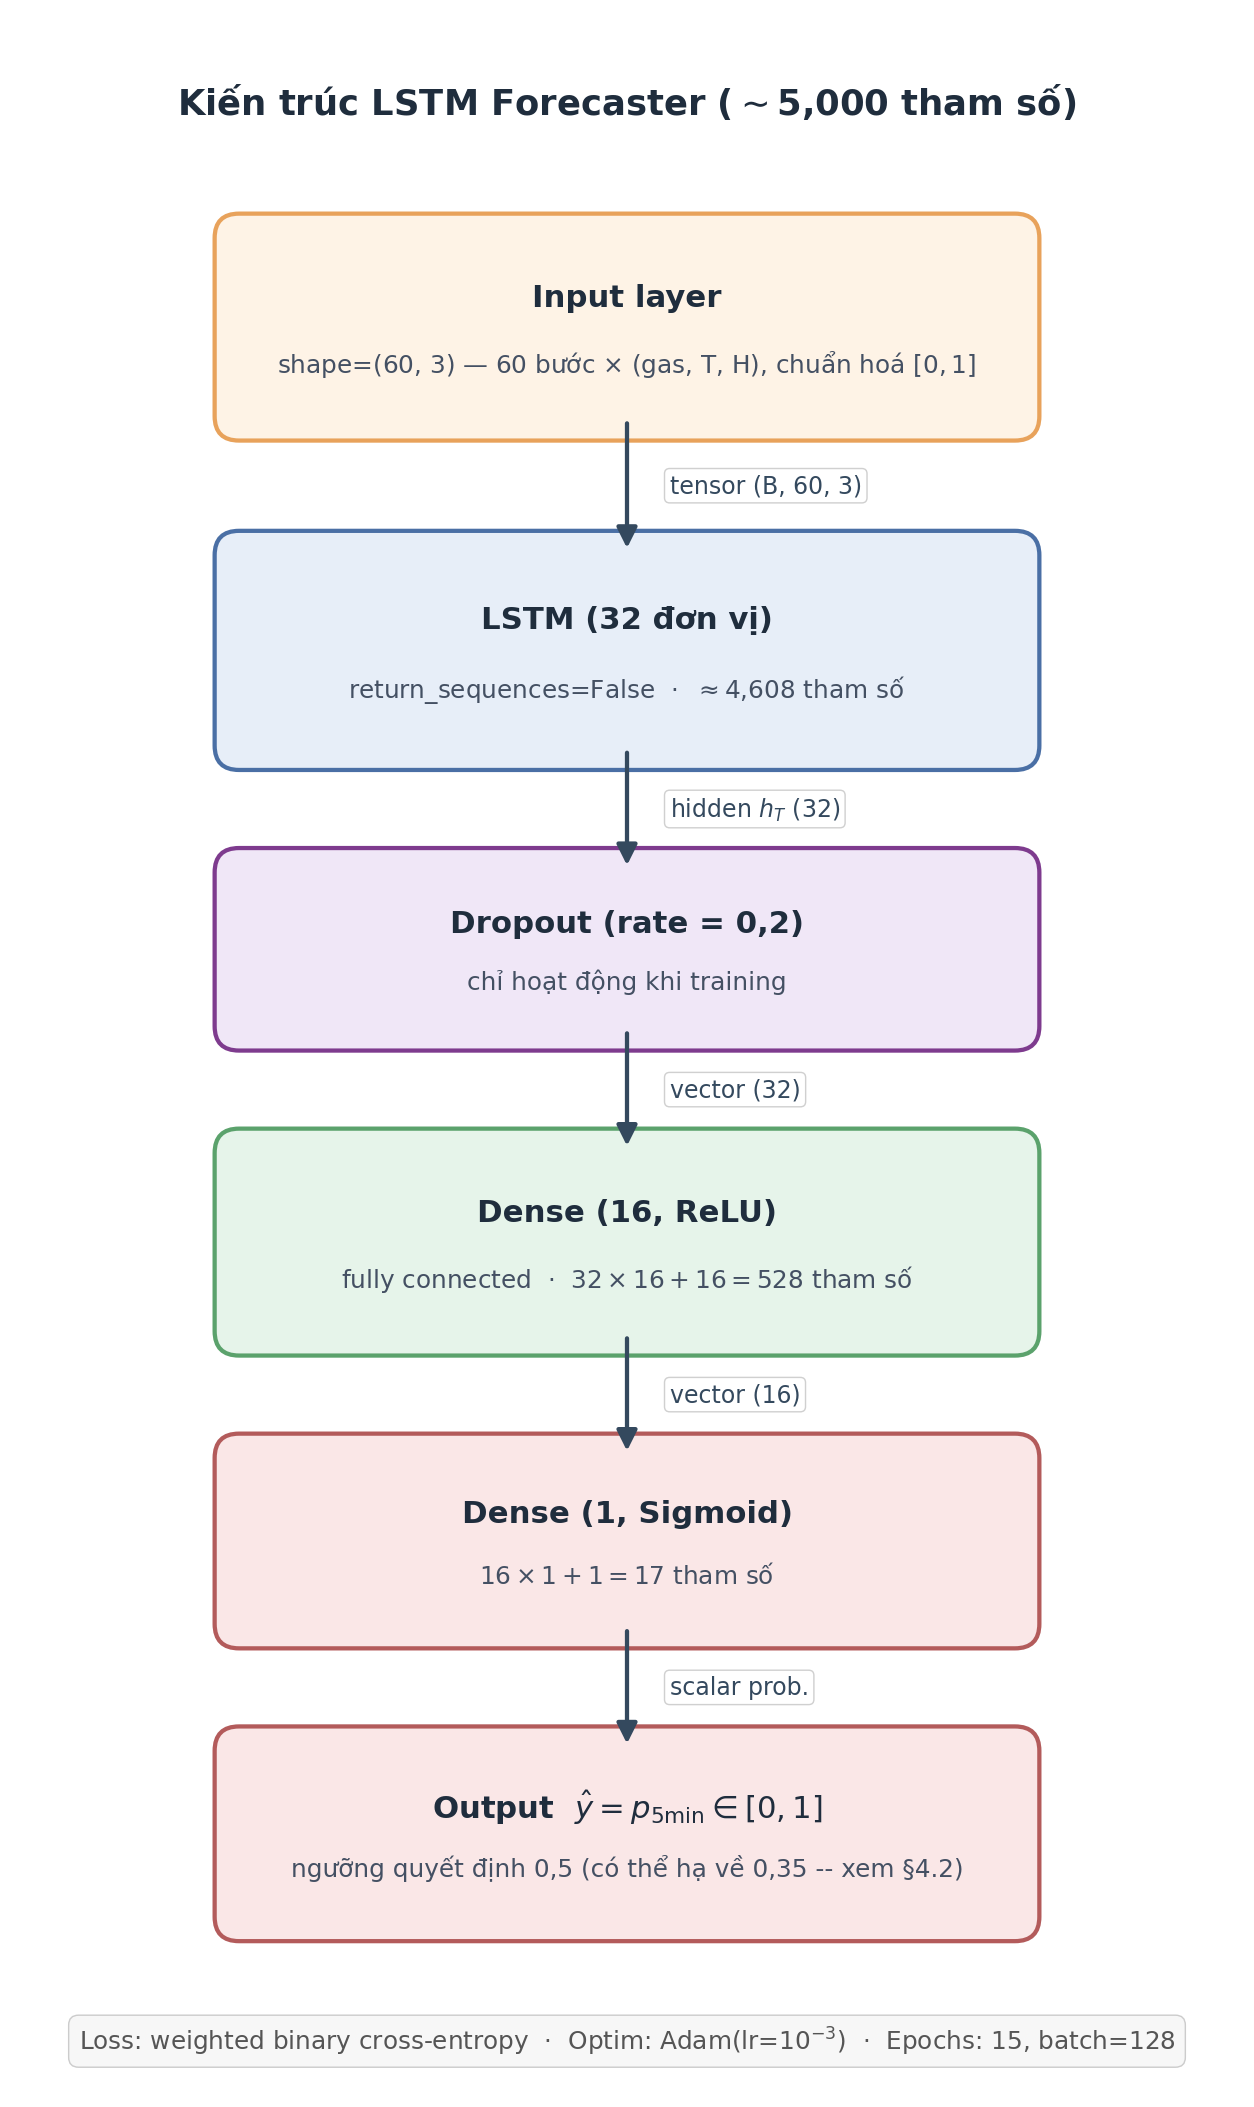
\includegraphics[width=0.62\linewidth]{lstm_arch.png}
  \captionof{figure}{Sơ đồ khối kiến trúc LSTM.}
  \label{fig:lstm_arch}
\end{center}

Trong các hệ thống xử lý dữ liệu theo luồng, mô hình LSTM cần có kích thước phù hợp để giảm thời gian suy luận và đáp ứng yêu cầu xử lý gần thời gian thực. Các thông số cụ thể như số bước thời gian đầu vào, số đặc trưng, ngưỡng dự báo và kiến trúc chi tiết của mô hình sẽ phụ thuộc vào bài toán triển khai cụ thể.

\section{Học tăng cường và thuật toán PPO}

Học tăng cường (Reinforcement Learning -- RL) là một hướng học máy trong đó một tác nhân học cách ra quyết định thông qua quá trình tương tác với môi trường. Tại mỗi bước, tác nhân quan sát trạng thái hiện tại, lựa chọn hành động, nhận phần thưởng và chuyển sang trạng thái mới. Qua nhiều lần tương tác, tác nhân học được chính sách hành động nhằm tối đa hóa tổng phần thưởng tích lũy.

\begin{center}
  
\includegraphics[width=0.65\textwidth]{rl_loop.png}
  \captionof{figure}{Vòng lặp tương tác giữa tác nhân và môi trường trong học tăng cường.}
  \label{fig:rl_loop}
\end{center}

Học tăng cường phù hợp với các bài toán ra quyết định tuần tự, trong đó hành động hiện tại có thể ảnh hưởng đến trạng thái tương lai. So với các luật điều khiển cố định, RL cho phép tác nhân học chính sách hành động thông qua dữ liệu tương tác và hàm thưởng được thiết kế theo mục tiêu của hệ thống.

\subsection{Mô hình MDP}

Bài toán RL thường được mô tả bằng Markov Decision Process (MDP), gồm năm thành phần $(\mathcal{S}, \mathcal{A}, \mathcal{P}, \mathcal{R}, \gamma)$:

\begin{itemize}
  \item $\mathcal{S}$: không gian trạng thái.
  \item $\mathcal{A}$: không gian hành động.
  \item $\mathcal{P}$: xác suất chuyển trạng thái.
  \item $\mathcal{R}$: hàm reward.
  \item $\gamma$: hệ số chiết khấu cho reward tương lai.
\end{itemize}

Trong một bài toán điều khiển, trạng thái có thể bao gồm các biến mô tả môi trường và trạng thái thiết bị; hành động có thể là các lựa chọn điều khiển rời rạc hoặc liên tục. Hàm reward được thiết kế để phản ánh mục tiêu mong muốn, chẳng hạn tăng độ an toàn, giảm chi phí hoặc hạn chế hành động không cần thiết.

\subsection{Proximal Policy Optimization}

Proximal Policy Optimization (PPO) là thuật toán policy gradient được sử dụng rộng rãi nhờ tính ổn định và khả năng triển khai thuận tiện \cite{schulman2017}. PPO cập nhật chính sách theo hướng cải thiện reward, đồng thời giới hạn mức thay đổi của chính sách sau mỗi lần cập nhật. Cơ chế này giúp quá trình học ổn định hơn so với việc cập nhật chính sách quá mạnh.

PPO thường được sử dụng trong các môi trường mô phỏng để huấn luyện tác nhân trước khi đánh giá hoặc triển khai trong hệ thống thực tế. Trong các bài toán có không gian hành động rời rạc, PPO có thể học cách chọn hành động phù hợp dựa trên trạng thái quan sát và tín hiệu phần thưởng từ môi trường.

\section{Docker và container hóa}

\techlogo{docker.jpg}{3cm}{Logo Docker}{fig:Docker_logo}

Docker là nền tảng container hóa cho phép đóng gói ứng dụng cùng thư viện, biến môi trường và cấu hình cần thiết vào các container độc lập. Mỗi container thường chạy một dịch vụ riêng, giúp giảm sự phụ thuộc vào môi trường cài đặt trên máy chủ.

Docker Compose là công cụ dùng để khai báo và quản lý nhiều Docker container thông qua một file cấu hình. Với các hệ thống gồm nhiều dịch vụ, Docker Compose giúp khởi động, dừng, cấu hình mạng và quản lý các container thuận tiện hơn.

Trong phạm vi triển khai thực nghiệm, hệ thống sử dụng Docker Compose để vận hành nhiều container. Docker Compose sẽ là công cụ điều phối các container trong cùng một môi trường chạy.

\section{Cơ sở dữ liệu và hiển thị dữ liệu}

\subsection{InfluxDB và PostgreSQL}

InfluxDB là cơ sở dữ liệu chuỗi thời gian, phù hợp với dữ liệu cảm biến được ghi liên tục theo timestamp. InfluxDB thường được dùng để lưu các bản ghi như nồng độ khí, nhiệt độ, độ ẩm, xác suất dự báo và hành động điều khiển.

\techlogo{influxdb.png}{3cm}{Logo InfluxDB}{fig:influxdb_logo}

PostgreSQL được dùng cho dữ liệu nghiệp vụ có cấu trúc rõ ràng hơn, chẳng hạn lịch sử cảnh báo và lịch sử hành động. Việc tách InfluxDB và PostgreSQL giúp mỗi loại dữ liệu được lưu ở công cụ phù hợp với cách truy vấn của nó: InfluxDB cho chuỗi thời gian, PostgreSQL cho dữ liệu quan hệ.

\techlogo{Postgresql.png}{3cm}{Logo Postgresql}{fig:postgresql_logo}

\subsection{Grafana, bảng điều khiển web và Telegram}

Grafana được dùng để trực quan hóa dữ liệu chuỗi thời gian và hỗ trợ quan sát trạng thái hệ thống trong quá trình thực nghiệm. Bảng điều khiển web có thể hiển thị dữ liệu hiện tại, đồ thị nồng độ khí, xác suất rủi ro và hành động của bộ điều khiển PPO.

\techlogo{grafana.jpg}{3cm}{Logo Grafana}{fig:grafana_logo}

Telegram Bot API được sử dụng như kênh cảnh báo cho người dùng. Khi hệ thống phát hiện nguy cơ hoặc bộ điều khiển chọn hành động cảnh báo, dịch vụ API có thể gửi thông báo đến Telegram kèm thông tin nồng độ khí, mức rủi ro và hành động hiện tại.

\techlogo{Telegram.png}{3cm}{Logo Telegram}{fig:Tele_logo}

\vspace{0.5em}

Tóm lại, chương này đã trình bày các nền tảng chính gồm IoT, giao thức truyền thông, xử lý luồng dữ liệu, LSTM, học tăng cường và PPO, cùng các công cụ lưu trữ/hiển thị dữ liệu. Các khái niệm này là cơ sở để chương tiếp theo mô tả cách hiện thực kiến trúc hệ thống và quy trình huấn luyện, đánh giá.
